\documentclass[10pt,oneside,swedish]{../lips}

%\usepackage[square]{natbib}\bibliographystyle{plainnat}\setcitestyle{numbers}
%\usepackage[round]{natbib}
\bibliographystyle{IEEEtran}

% Configure the document
\title{Kravspecifikation Taxibil}
\author{Projektgrupp 13}
\date{16 september 2022}
\version{1.0.1}

\reviewed{Johan Klasén}{14 september 2022}
\approved{Anders Nilsson}{15 september 2022}

\begin{document}
\projecttitle{Taxibil-robot}

\groupname{Projektgrupp 13}
\groupemail{TSEA29_2022HT_E7-Grupp13@groups.liu.se}
\groupwww{https://gitlab.liu.se/da-proj/microcomputer-project-laboratory-d/2022/g13}

\coursecode{TSEA29}
\coursename{Konstruktion med mikrodatorer}

\orderer{Anders Nilsson, ISY, Linköpings universitet}
\ordererphone{013-28 26 35}
\ordereremail{anders.p.nilsson@liu.se}

\customer{Anders Nilsson, ISY, Linköpings universitet}
\customerphone{013-28 26 35}
\customeremail{anders.p.nilsson@liu.se}

\courseresponsible{Anders Nilsson, ISY, Linköpings universitetn}
\courseresponsiblephone{013-28 26 35}
\courseresponsibleemail{anders.p.nilsson@liu.se}

\supervisor{Peter Johansson}
\supervisorphone{013-28 1345}
\supervisoremail{peter.a.johansson@liu.se}

\smalllogo{../Figures/LiU_primary_black} % Page header logo, filename
\biglogo{../Figures/logo} % Front page logo, filename

\cfoot{\thepage}
\begin{document}
\maketitle

\cleardoublepage
\makeprojectid

\begin{center}
  \Large Projektdeltagare
\end{center}
\begin{center}
  \begin{tabular}{|l|l|l|l|}
    \hline
    \textbf{Namn} & \textbf{Ansvar} & \textbf{Telefon} & \textbf{E-post}\\
    \hline
    Linus Thorsell & Projektledare & 0765612171 & linth181@student.liu.se\\
    \hline
    Oscar Sandell & Testansvarig & 0709416866 & oscsa604@student.liu.se\\
    \hline
    Hannes Nöranger & Utvecklare & 0733118779 & hanno696@student.liu.se\\
    \hline
    Johan Klasén & Dokumentansvarig & 0730982555 & johkl473@student.liu.se\\
    \hline
    Zackarias Wadströmer & Utvecklare & 0706142029 & zacwa923@student.liu.se\\
    \hline
    Thomas Pilotti Wiger & Konstruktionsansvarig & 0761708593 & thopi836@student.liu.se\\
    \hline
  \end{tabular}
\end{center}


\cleardoublepage
\tableofcontents

\cleardoublepage
\section*{Dokumenthistorik}
\begin{tabular}{p{.06\textwidth}|p{.1\textwidth}|p{.44\textwidth}|p{.13\textwidth}|p{.13\textwidth}} 
  \multicolumn{1}{c}{\bfseries Version} & 
  \multicolumn{1}{|c}{\bfseries Datum} & 
  \multicolumn{1}{|c}{\bfseries Utförda ändringar} & 
  \multicolumn{1}{|c}{\bfseries Utförda av} & 
  \multicolumn{1}{|c}{\bfseries Granskad}\\
  \hline
  \hline
  1.0 & 2022-09-15 & Första versionen & JK &    \\
  \hline
  0.3 & 2022-09-14 & Tredje utkast & JK & TW \\
  \hline
  0.2 & 2022-09-12 & Andra utkast & Gruppen & Gruppen \\
  \hline
  0.1 & 2022-09-08 & Första utkast & Gruppen & Gruppen \\
  \hline
\end{tabular}

\cleardoublepage
\pagenumbering{arabic}\cfoot{\thepage}

\section{Inledning}
\label{sec:inledning}

Presenterade i denna kravspecifikation är alla de krav sammanställda för projektet och dess genomförande.

\begin{figure}[htbp]
  \centering
  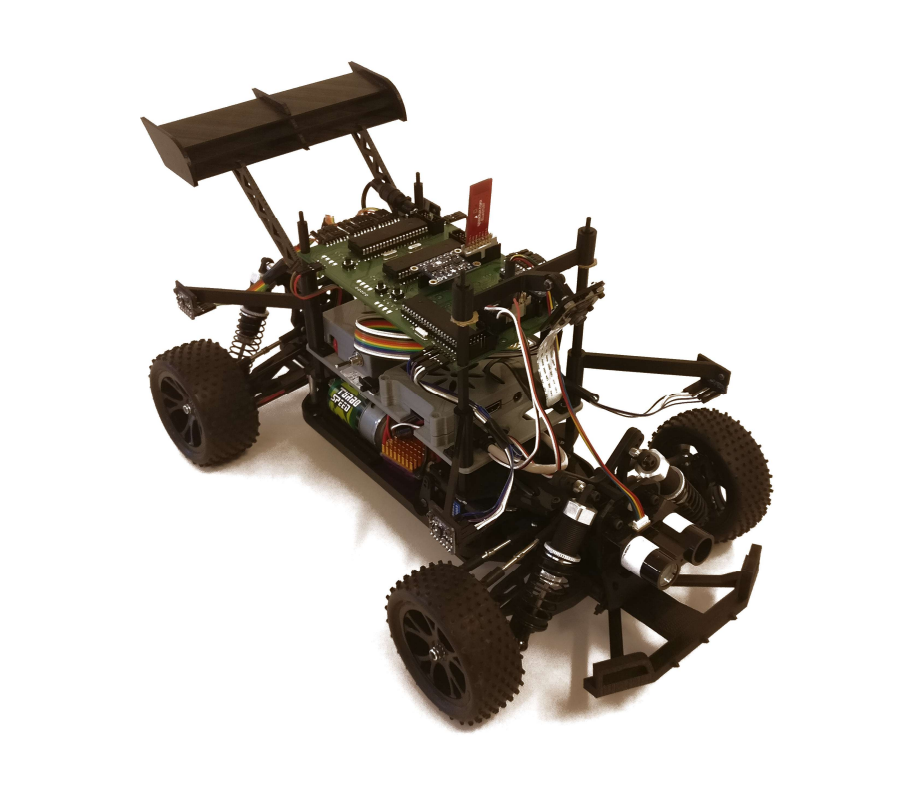
\includegraphics[width=.7\textwidth]{../Figures/exempelbil}
  \caption{Ett exempel på en bil med diverse sensorer}
  \label{fig:bil}
\end{figure}\textbf{}

Kraven presenteras på formen:
\begin{longtable}{|c|p{17mm}|p{100mm}|c|}
  \hline
  Kravnummer & Version &  Kravtext för krav nr X & Prioritet\\
  \hline
\end{longtable}
%\begin{requirements}
%  \requirementno & Orginal & Alla dokument skall uppfylla instruktioner
%  beskrivna i \cite{spraknamnd:2000} & 1\\
%\end{requirements}

\subsection{Parter}
Projektet kommer utföras av en grupp studenter, även benämnd “gruppen” eller “projektgruppen”, under handledning av Peter Johansson härefter benämnd “handledaren” till förmån för Anders Nilsson också känd som “kunden”.

\subsection{Syfte och mål}
Projektets syfte är konstruktionen av en autonom taxibil. Arbetet kommer framförallt vara att utveckla systemet och den tekniska designen. 

\subsection{Användning}
Produkten används fritt av kunden efter leverans.

\subsection{Bakgrundsinformation}
Kunden vill undersöka möjligheterna att konstruera en autonom bil. Bilen ska kunna köra autonomt från en punkt till en annan i ett känt vägnät utan att kollidera med eventuella hinder på vägen. 
För att utvärdera hur en sådan bil kan konstrueras har kunden anordnat en tävling där flera prototyper ska delta för att utvärdera olika konstruktionsalternativ.

\subsection{Definitioner}
Prioritetsnivåer \cite{lect3}:
\begin{itemize}
  \item 1. Grundkrav, ska uppfyllas vid beslutspunkt 5.
  \item 2. Extra krav, ska uppfyllas om det finns tid kvar då grundkraven är utförda.
  \item 3. Krav på framtida utbyggnad, uppfylls om tid finns då samtliga krav med prioritet 1 och 2 är uppfyllda.
\end{itemize}

Autonom - Utan externt inflytande.\\
Bil, taxibil, robot - Den produkt som projektet utvecklar.\\
Köruppdrag, uppdrag - Att i en bana hämta upp passagerare och föra dem till sin destination.\\
Telemetri - Mätdata såsom avstånd till vägkant eller synbara hinder, avlagd sträcka, styrbeslut och styrdata till den bärbara datorn.\\


\section{Översikt av systemet}
En kortare översikt av det konstruerade systemet.
\begin{figure}[htbp]
  \centering
  
\includegraphics[width=.7\textwidth]{../Figures/placeholder}
  \caption{Denna bild visar en översikt av systemet.}
  \label{fig:oversikt}
\end{figure}

\subsection{Grov beskrivning av produkten}
Produkten är en autonom taxibil som kan navigera sig genom ett vägnät i enlighet med angivna krav. Tillkommer gör mjukvara för att till viss grad styra samt inspektera systemet.

\subsection{Produktkomponenter}
Produkten utgörs av en färdigbyggd bil samt mjukvara för att kontrollera den. 

\subsection{Beroenden till andra system}
Inget beroende i nuläget utöver Python.

\subsection{Ingående delsystem}
Produkten kommer bestå av en färdigkonstruerad bil med motorer och servon. 
Den kommer även bestå av en kommunikationsmodul, styrmodul, sensormodul samt en extern applikation.

\subsection{Avgränsningar}
Det autonoma fordonet ska endast förväntas navigera en väl definierad bana. Banan designas i samråd med de övriga grupperna som deltar i tävlingen och beskrivs i ingående detalj i dokumentet Banspecifikation \cite{banspec}.

\subsection{Generella krav på hela systemet}\label{genreq}
En lista på generella krav som gäller hela systemet.

\begin{requirements}
  \ref{genreq}.\requirementno & Orginal & Bilen ska köra autonomt från en punkt till en annan i ett känt vägnät enligt banspecifikation \cite{banspec}. & 1\\
  \hline
  \ref{genreq}.\requirementno & Original & Bilen ska inte kollidera med hinder på vägen genom att bilen stannar tills det att hindret tas bort. & 1\\
  \hline
  \ref{genreq}.\requirementno & Original & Bilen ska stanna och hämta/upp släppa av passagerare vid en enligt banspecifikationen\cite{banspec} känd punkt på banan. & 1\\
  \hline
  \ref{genreq}.\requirementno & Original & text & 1\\
  \hline
  \ref{genreq}.\requirementno & Original & text & 1\\
  \hline
  \ref{genreq}.\requirementno & Original & text & 1\\
  \hline
  \ref{genreq}.\requirementno & Original & text & 1\\
  \hline
  \ref{genreq}.\requirementno & Original & text & 1\\
  \hline
\end{requirements}

\section{Delsystem 1 Kommunikationsmodul}
Systemets kommunikationsmodul ska vara den hub på roboten som kommunicerar med den externa datorn. Den ska ta emot data från en extern källa som ska påverka roboten.

\subsection{Krav för delsystem 1}\label{delsys1req}

\begin{requirements}
  \ref{delsys1req}.\requirementno & Orginal & Bilen ska kommunicera med en Extern Laptop. & 1\\
  \hline
  \ref{delsys1req}.\requirementno & Orginal & Bilen ska fortlöpande skicka mätdata såsom avstånd till vägkant eller synbara hinder, avlagd sträcka etc, samt styrbeslut och styrdata. & 1\\
  \hline
\end{requirements}

\section{Delsystem 2 Styrmodul}
Styrmodulens uppgift är att driva taxibilen framåt så att den kan utföra uppdraget. Detta genom att kontrollera de olika aktuatorerna på roboten så som motorer och styrning. Modulen får data från kommunikationsmodulen och styr roboten därefter.

\subsection{Krav för delsystem 2}\label{delsys2req}

\begin{requirements}
  \ref{delsys2req}.\requirementno & Orginal & Bilen ska kommunicera med en Extern Laptop. & 1\\
  \hline
  \ref{delsys2req}.\requirementno & Orginal & Bilen ska fortlöpande skicka mätdata såsom avstånd till vägkant eller synbara hinder, avlagd sträcka etc, samt styrbeslut och styrdata. & 1\\
  \hline
\end{requirements}

\section{Delsystem 3 Sensormodul}
Denna modul ska ansvara för att fixa fram mätdata från sensorerna och sedan skicka den till kommunikationsmodulen.

\subsection{Krav för delsystem 3}\label{delsys3req}

\begin{requirements}
  \ref{delsys3req}.\requirementno & Orginal & Bilen ska kommunicera med en Extern Laptop. & 1\\
  \hline
  \ref{delsys3req}.\requirementno & Orginal & Bilen ska fortlöpande skicka mätdata såsom avstånd till vägkant eller synbara hinder, avlagd sträcka etc, samt styrbeslut och styrdata. & 1\\
  \hline
\end{requirements}

\section{Delsystem 4 Extern Applikation}
Denna applikation skall ta emot data från kommunikationsmodulen på Taxibilen och visa relevant telemetridata på gränssnittet. Denna skall även kunna användas för att manuellt styra och ändra inställningar på Taxibilen.

\subsection{Krav för delsystem 4}\label{delsys4req}

\begin{requirements}
  \ref{delsys4req}.\requirementno & Orginal & Bilen ska kommunicera med en Extern Laptop. & 1\\
  \hline
  \ref{delsys4req}.\requirementno & Orginal & Bilen ska fortlöpande skicka mätdata såsom avstånd till vägkant eller synbara hinder, avlagd sträcka etc, samt styrbeslut och styrdata. & 1\\
  \hline
\end{requirements}

\section{Utvecklingsmetodik}
Ett krav från beställaren är att utveckling av produkten ska ske enligt den så kallade LIPS-modellen \cite{lips-modellen}. LIPS-modellen beskriver övergripande vilka delmoment projektet ska delas upp i för att få ett bra flöde under projekttiden. \\
I detta ingår även en viss mängd planeringsmoment och dokumentation som ska ske löpande under projekttiden. Dessa delmoment listas nedan under rubrikerna \emph{Leveranskrav och delleveranser} och \emph{Dokumentation}. \\
Projektet ska även utföras inom en strikt budgeterad tidsram på 160 arbetstimmar/person efter det att en godkänd projektplan har levererats och godkänts av beställaren.

\subsection{Krav för utvecklingsmetodiken}
\begin{requirements}
  \requirementno & Orginal & Kravtext & 1\\
\end{requirements}

\section{Leveranskrav och delleveranser} 
Produkten som förväntas levereras till beställaren består av en fungerande autonom taxibil med tillhörande teknisk dokumentation och användaranvisningar.\\
Projektgruppen förväntas möta följande leveranser till beställaren.

\begin{requirements}
  \requirementno & Orginal & Kravtext & Bas\\
\end{requirements}

\section{Dokumentation} 
Dokument som projektgruppen kommer tillhandahålla presenteras i \ref{tab:doks} nedan.
\begin{table}[htbp]
  \centering
  \caption{Dokument som skall produceras}
  \label{tab:doks}
  \begin{tabular}{|p{22mm}|l|p{80mm}|l|p{17mm}|}
    \hline
    Dokument & Språk & Syfte & Målgrupp & Format\\
    \hline
    Systemskiss & Svenska & Övergripande modell hur produkten ska designas. Ska innehålla modulindelning av systemet och ett preliminärt blockschema. & Kund & Pdf\\
    \hline
    Projektplan & Svenska & Planering för projektets villkor och utförande samt övergripande fördelning av den tillgängliga projekttiden i form av aktiviteter. & Kund & Pdf\\
    \hline
    Tidsplan & Svenska & Detaljerat schema över hur projektmedlemmarna kommer fördela tillgängliga arbetstimmar under projekttiden utgående från aktiviteterna i projektplanen. & Kund & Excel-dokument\\
    \hline
    Tidsrapportering & Svenska & Löpande redovisning av tidsanvändning till kunden. & Kund & Markdown-filer\\
    \hline
    Design-specifikation & Svenska & Förfining av systemskissen på tydlig detaljnivå över hur produkten ska konstrueras. Ska innehålla krets- och flödesscheman. & Handledaren & Pdf\\
    \hline
    Teknisk dokumentation & Svenska & Komplett beskrivning av hur produkten är konstruerad. & Kund & Pdf\\
    \hline
    Användar-handledning & Svenska & Tydliga instruktioner hur man använder produkten. & Kund & Pdf\\
    \hline
    Efterstudie & Svenska & Sammanställning hur projektgruppen upplevde utförandet av av arbetet. & Kund & Pdf\\
    \hline
  \end{tabular}  
\end{table}

\clearpage
\bibliography{references}

\cleardoublepage

\end{document}

%%% Local Variables:
%%% mode: latex
%%% TeX-master: t
%%% End:
